\documentclass{standalone}
\makeatletter\AtBeginDocument{\@buildstepset{1,2,3,4}}\makeatother
\usepackage{tikz}
\usetikzlibrary{intersections, calc}
\usepackage{hsbcommon}
\begin{document}
    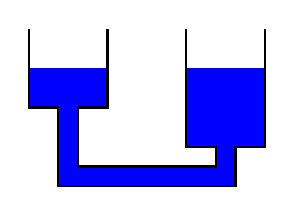
\begin{tikzpicture}[scale=0.5]
        \path[fill=blue] (0,-2) -- (0,-3) -- (0.75,-3) -- (0.75,-5) -- (5.25,-5) -- (5.25,-4) -- (6,-4) -- (6,-2) -- (4,-2) -- (4,-4) -- (4.75,-4) -- (4.75,-4.5) -- (1.25,-4.5) -- (1.25,-3) -- (2,-3) -- (2,-2) -- cycle;
        \path[draw,thick] (0,-1) -- (0,-3) -- (0.75,-3) -- (0.75,-5) -- (5.25,-5) -- (5.25,-4) -- (6,-4) -- (6,-1);
        \path[draw,thick] (4,-1) -- (4,-4) -- (4.75,-4) -- (4.75,-4.5) -- (1.25,-4.5) -- (1.25,-3) -- (2,-3) -- (2,-1);
    \end{tikzpicture}
\end{document}
